% Created by tikzDevice version 0.12.6 on 2024-11-13 12:24:15
% !TEX encoding = UTF-8 Unicode
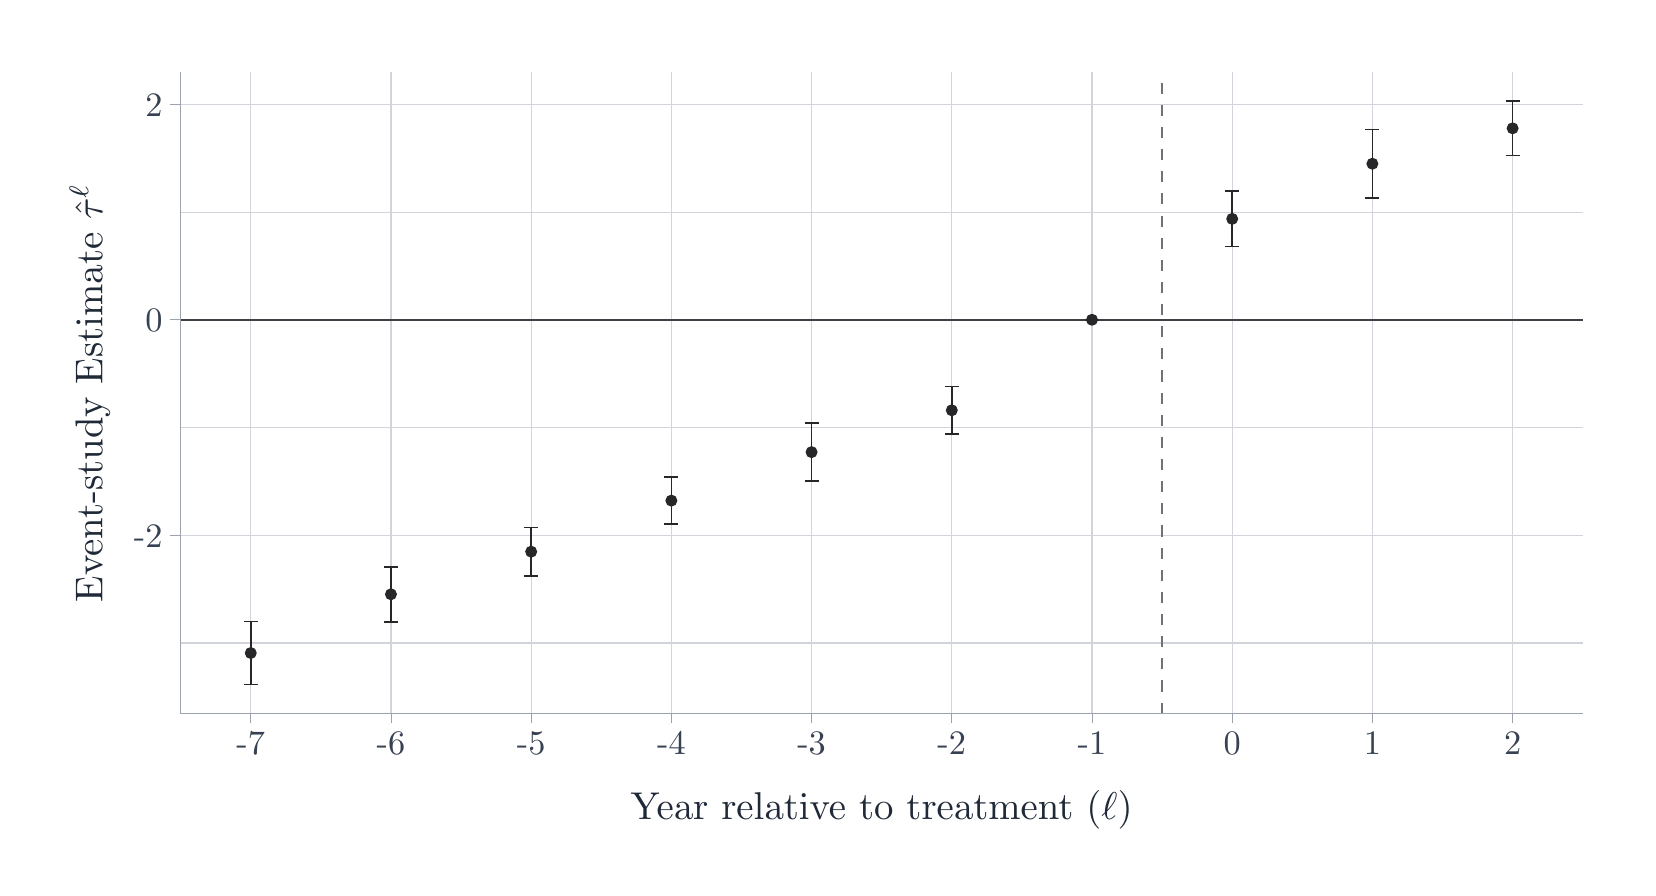
\begin{tikzpicture}[x=1pt,y=1pt]
\definecolor{fillColor}{RGB}{255,255,255}
\path[use as bounding box,fill=fillColor] (0,0) rectangle (578.16,303.53);
\begin{scope}
\path[clip] (  0.00,  0.00) rectangle (578.16,303.53);
\definecolor{drawColor}{RGB}{255,255,255}

\path[draw=drawColor,line width= 0.7pt,line join=round,line cap=round,fill=fillColor] (  0.00,  0.00) rectangle (578.16,303.53);
\end{scope}
\begin{scope}
\path[clip] ( 55.03, 55.65) rectangle (562.16,287.53);
\definecolor{drawColor}{RGB}{255,255,255}
\definecolor{fillColor}{RGB}{255,255,255}

\path[draw=drawColor,line width= 0.7pt,line join=round,line cap=round,fill=fillColor] ( 55.03, 55.65) rectangle (562.16,287.53);
\definecolor{drawColor}{RGB}{209,213,219}

\path[draw=drawColor,line width= 0.4pt,line join=round] ( 55.03, 81.19) --
	(562.16, 81.19);

\path[draw=drawColor,line width= 0.4pt,line join=round] ( 55.03,159.05) --
	(562.16,159.05);

\path[draw=drawColor,line width= 0.4pt,line join=round] ( 55.03,236.90) --
	(562.16,236.90);

\path[draw=drawColor,line width= 0.4pt,line join=round] ( 55.03,120.12) --
	(562.16,120.12);

\path[draw=drawColor,line width= 0.4pt,line join=round] ( 55.03,197.98) --
	(562.16,197.98);

\path[draw=drawColor,line width= 0.4pt,line join=round] ( 55.03,275.83) --
	(562.16,275.83);

\path[draw=drawColor,line width= 0.4pt,line join=round] ( 80.61, 55.65) --
	( 80.61,287.53);

\path[draw=drawColor,line width= 0.4pt,line join=round] (131.27, 55.65) --
	(131.27,287.53);

\path[draw=drawColor,line width= 0.4pt,line join=round] (181.94, 55.65) --
	(181.94,287.53);

\path[draw=drawColor,line width= 0.4pt,line join=round] (232.60, 55.65) --
	(232.60,287.53);

\path[draw=drawColor,line width= 0.4pt,line join=round] (283.26, 55.65) --
	(283.26,287.53);

\path[draw=drawColor,line width= 0.4pt,line join=round] (333.93, 55.65) --
	(333.93,287.53);

\path[draw=drawColor,line width= 0.4pt,line join=round] (384.59, 55.65) --
	(384.59,287.53);

\path[draw=drawColor,line width= 0.4pt,line join=round] (435.25, 55.65) --
	(435.25,287.53);

\path[draw=drawColor,line width= 0.4pt,line join=round] (485.91, 55.65) --
	(485.91,287.53);

\path[draw=drawColor,line width= 0.4pt,line join=round] (536.58, 55.65) --
	(536.58,287.53);
\definecolor{drawColor}{RGB}{63,63,70}

\path[draw=drawColor,line width= 0.6pt,line join=round] ( 55.03,197.98) -- (562.16,197.98);
\definecolor{drawColor}{RGB}{113,113,122}

\path[draw=drawColor,line width= 0.6pt,dash pattern=on 4pt off 4pt ,line join=round] (409.92, 55.65) -- (409.92,287.53);
\definecolor{drawColor}{RGB}{39,39,42}
\definecolor{fillColor}{RGB}{39,39,42}

\path[draw=drawColor,line width= 0.4pt,line join=round,line cap=round,fill=fillColor] ( 80.61, 77.56) circle (  1.96);

\path[draw=drawColor,line width= 0.4pt,line join=round,line cap=round,fill=fillColor] (131.27, 98.79) circle (  1.96);

\path[draw=drawColor,line width= 0.4pt,line join=round,line cap=round,fill=fillColor] (181.94,114.18) circle (  1.96);

\path[draw=drawColor,line width= 0.4pt,line join=round,line cap=round,fill=fillColor] (232.60,132.63) circle (  1.96);

\path[draw=drawColor,line width= 0.4pt,line join=round,line cap=round,fill=fillColor] (283.26,150.15) circle (  1.96);

\path[draw=drawColor,line width= 0.4pt,line join=round,line cap=round,fill=fillColor] (333.93,165.27) circle (  1.96);

\path[draw=drawColor,line width= 0.4pt,line join=round,line cap=round,fill=fillColor] (384.59,197.98) circle (  1.96);

\path[draw=drawColor,line width= 0.4pt,line join=round,line cap=round,fill=fillColor] (435.25,234.44) circle (  1.96);

\path[draw=drawColor,line width= 0.4pt,line join=round,line cap=round,fill=fillColor] (485.91,254.36) circle (  1.96);

\path[draw=drawColor,line width= 0.4pt,line join=round,line cap=round,fill=fillColor] (536.58,267.16) circle (  1.96);

\path[draw=drawColor,line width= 0.6pt,line join=round] ( 78.08, 88.92) --
	( 83.15, 88.92);

\path[draw=drawColor,line width= 0.6pt,line join=round] ( 80.61, 88.92) --
	( 80.61, 66.19);

\path[draw=drawColor,line width= 0.6pt,line join=round] ( 78.08, 66.19) --
	( 83.15, 66.19);

\path[draw=drawColor,line width= 0.6pt,line join=round] (128.74,108.76) --
	(133.81,108.76);

\path[draw=drawColor,line width= 0.6pt,line join=round] (131.27,108.76) --
	(131.27, 88.82);

\path[draw=drawColor,line width= 0.6pt,line join=round] (128.74, 88.82) --
	(133.81, 88.82);

\path[draw=drawColor,line width= 0.6pt,line join=round] (179.40,122.93) --
	(184.47,122.93);

\path[draw=drawColor,line width= 0.6pt,line join=round] (181.94,122.93) --
	(181.94,105.42);

\path[draw=drawColor,line width= 0.6pt,line join=round] (179.40,105.42) --
	(184.47,105.42);

\path[draw=drawColor,line width= 0.6pt,line join=round] (230.07,141.07) --
	(235.13,141.07);

\path[draw=drawColor,line width= 0.6pt,line join=round] (232.60,141.07) --
	(232.60,124.18);

\path[draw=drawColor,line width= 0.6pt,line join=round] (230.07,124.18) --
	(235.13,124.18);

\path[draw=drawColor,line width= 0.6pt,line join=round] (280.73,160.60) --
	(285.80,160.60);

\path[draw=drawColor,line width= 0.6pt,line join=round] (283.26,160.60) --
	(283.26,139.70);

\path[draw=drawColor,line width= 0.6pt,line join=round] (280.73,139.70) --
	(285.80,139.70);

\path[draw=drawColor,line width= 0.6pt,line join=round] (331.39,173.90) --
	(336.46,173.90);

\path[draw=drawColor,line width= 0.6pt,line join=round] (333.93,173.90) --
	(333.93,156.64);

\path[draw=drawColor,line width= 0.6pt,line join=round] (331.39,156.64) --
	(336.46,156.64);

\path[draw=drawColor,line width= 0.6pt,line join=round] (382.05,197.98) --
	(387.12,197.98);

\path[draw=drawColor,line width= 0.6pt,line join=round] (384.59,197.98) --
	(384.59,197.98);

\path[draw=drawColor,line width= 0.6pt,line join=round] (382.05,197.98) --
	(387.12,197.98);

\path[draw=drawColor,line width= 0.6pt,line join=round] (432.72,244.45) --
	(437.78,244.45);

\path[draw=drawColor,line width= 0.6pt,line join=round] (435.25,244.45) --
	(435.25,224.43);

\path[draw=drawColor,line width= 0.6pt,line join=round] (432.72,224.43) --
	(437.78,224.43);

\path[draw=drawColor,line width= 0.6pt,line join=round] (483.38,266.79) --
	(488.45,266.79);

\path[draw=drawColor,line width= 0.6pt,line join=round] (485.91,266.79) --
	(485.91,241.94);

\path[draw=drawColor,line width= 0.6pt,line join=round] (483.38,241.94) --
	(488.45,241.94);

\path[draw=drawColor,line width= 0.6pt,line join=round] (534.04,276.99) --
	(539.11,276.99);

\path[draw=drawColor,line width= 0.6pt,line join=round] (536.58,276.99) --
	(536.58,257.32);

\path[draw=drawColor,line width= 0.6pt,line join=round] (534.04,257.32) --
	(539.11,257.32);
\end{scope}
\begin{scope}
\path[clip] (  0.00,  0.00) rectangle (578.16,303.53);
\definecolor{drawColor}{RGB}{156,163,175}

\path[draw=drawColor,line width= 0.3pt,line join=round] ( 55.03, 55.65) --
	( 55.03,287.53);
\end{scope}
\begin{scope}
\path[clip] (  0.00,  0.00) rectangle (578.16,303.53);
\definecolor{drawColor}{RGB}{55,65,81}

\node[text=drawColor,anchor=base east,inner sep=0pt, outer sep=0pt, scale=  1.24] at ( 48.73,115.84) {-2};

\node[text=drawColor,anchor=base east,inner sep=0pt, outer sep=0pt, scale=  1.24] at ( 48.73,193.69) {0};

\node[text=drawColor,anchor=base east,inner sep=0pt, outer sep=0pt, scale=  1.24] at ( 48.73,271.55) {2};
\end{scope}
\begin{scope}
\path[clip] (  0.00,  0.00) rectangle (578.16,303.53);
\definecolor{drawColor}{RGB}{156,163,175}

\path[draw=drawColor,line width= 0.3pt,line join=round] ( 51.53,120.12) --
	( 55.03,120.12);

\path[draw=drawColor,line width= 0.3pt,line join=round] ( 51.53,197.98) --
	( 55.03,197.98);

\path[draw=drawColor,line width= 0.3pt,line join=round] ( 51.53,275.83) --
	( 55.03,275.83);
\end{scope}
\begin{scope}
\path[clip] (  0.00,  0.00) rectangle (578.16,303.53);
\definecolor{drawColor}{RGB}{156,163,175}

\path[draw=drawColor,line width= 0.3pt,line join=round] ( 55.03, 55.65) --
	(562.16, 55.65);
\end{scope}
\begin{scope}
\path[clip] (  0.00,  0.00) rectangle (578.16,303.53);
\definecolor{drawColor}{RGB}{156,163,175}

\path[draw=drawColor,line width= 0.3pt,line join=round] ( 80.61, 52.15) --
	( 80.61, 55.65);

\path[draw=drawColor,line width= 0.3pt,line join=round] (131.27, 52.15) --
	(131.27, 55.65);

\path[draw=drawColor,line width= 0.3pt,line join=round] (181.94, 52.15) --
	(181.94, 55.65);

\path[draw=drawColor,line width= 0.3pt,line join=round] (232.60, 52.15) --
	(232.60, 55.65);

\path[draw=drawColor,line width= 0.3pt,line join=round] (283.26, 52.15) --
	(283.26, 55.65);

\path[draw=drawColor,line width= 0.3pt,line join=round] (333.93, 52.15) --
	(333.93, 55.65);

\path[draw=drawColor,line width= 0.3pt,line join=round] (384.59, 52.15) --
	(384.59, 55.65);

\path[draw=drawColor,line width= 0.3pt,line join=round] (435.25, 52.15) --
	(435.25, 55.65);

\path[draw=drawColor,line width= 0.3pt,line join=round] (485.91, 52.15) --
	(485.91, 55.65);

\path[draw=drawColor,line width= 0.3pt,line join=round] (536.58, 52.15) --
	(536.58, 55.65);
\end{scope}
\begin{scope}
\path[clip] (  0.00,  0.00) rectangle (578.16,303.53);
\definecolor{drawColor}{RGB}{55,65,81}

\node[text=drawColor,anchor=base,inner sep=0pt, outer sep=0pt, scale=  1.24] at ( 80.61, 40.78) {-7};

\node[text=drawColor,anchor=base,inner sep=0pt, outer sep=0pt, scale=  1.24] at (131.27, 40.78) {-6};

\node[text=drawColor,anchor=base,inner sep=0pt, outer sep=0pt, scale=  1.24] at (181.94, 40.78) {-5};

\node[text=drawColor,anchor=base,inner sep=0pt, outer sep=0pt, scale=  1.24] at (232.60, 40.78) {-4};

\node[text=drawColor,anchor=base,inner sep=0pt, outer sep=0pt, scale=  1.24] at (283.26, 40.78) {-3};

\node[text=drawColor,anchor=base,inner sep=0pt, outer sep=0pt, scale=  1.24] at (333.93, 40.78) {-2};

\node[text=drawColor,anchor=base,inner sep=0pt, outer sep=0pt, scale=  1.24] at (384.59, 40.78) {-1};

\node[text=drawColor,anchor=base,inner sep=0pt, outer sep=0pt, scale=  1.24] at (435.25, 40.78) {0};

\node[text=drawColor,anchor=base,inner sep=0pt, outer sep=0pt, scale=  1.24] at (485.91, 40.78) {1};

\node[text=drawColor,anchor=base,inner sep=0pt, outer sep=0pt, scale=  1.24] at (536.58, 40.78) {2};
\end{scope}
\begin{scope}
\path[clip] (  0.00,  0.00) rectangle (578.16,303.53);
\definecolor{drawColor}{RGB}{31,41,55}

\node[text=drawColor,anchor=base,inner sep=0pt, outer sep=0pt, scale=  1.40] at (308.59, 17.36) {Year relative to treatment ($\ell$)};
\end{scope}
\begin{scope}
\path[clip] (  0.00,  0.00) rectangle (578.16,303.53);
\definecolor{drawColor}{RGB}{31,41,55}

\node[text=drawColor,rotate= 90.00,anchor=base,inner sep=0pt, outer sep=0pt, scale=  1.40] at ( 27.00,171.59) {Event-study Estimate $\hat{\tau}^{\ell}$};
\end{scope}
\end{tikzpicture}
